\chapter{Metodologia Proposta}
\label{chap3}
Todos os scripts desenvolvidos estão contidos no Apêndice \ref{appendice} e no diretório do  \href{https://github.com/lucascbarbosa/lstm-control-waam}{Github}.
\section{Geração dos dados}
\subsection{Simulação}
Os dados provenientes da simulação descrita na seção \ref{sec:simulation}, descrevem um sistema MIMO cujas entradas são a WFS $f$ e a corrente de referência da fonte $Ir$ e as saídas são a largura efetiva $w_e$ e a altura $h$ do cordão. Os valores das constantes utilizadas na simulação estão descritos na tabela \ref{tab:params_simulation} e são inicializados no script presente na seção \ref{code:gmaw_process}. Esses valores foram retirados de \cite{bendia2021multivariable}.

\begin{table}[hbt!]
    \centering
    \begin{tabular}{|c|c|}
    \hline
    Constante & Valor \\
    \hline
    $\eta$ & 0.655 \\
    \hline
    $\eta_d$ & 0.958 \\
    \hline
    $E_a$ & 723.2561 \\
    \hline
    $V_o$ & 5.1782 \\
    \hline
    $R_a$ & 0.0201 \\
    \hline
    $R_s$ & 0.004 \\
    \hline
    $L_s$ & 0.00014 \\
    \hline
    $V_{oc}$ & 31 \\
    \hline
    $k_v$ & 10 \\
    \hline
    $l_c$ & 0.01 \\
    \hline
    $v$ & 0.12 \\
    \hline
    $\Delta T$ & 1300 \\
    \hline
    $\rho$ & 0.1319 \\
    \hline
    $k$ & 24 \\
    \hline
    $\alpha$ & 7.79e-6 \\
    \hline
    $C_1$ & 3.2634e-10 \\
    \hline
    $C_2$ & 1.1836e-9 \\
    \hline
    $r_w$ & 0.0006 \\
    \hline
    $l_{so}$ & 0.0041 \\
    \hline
    $f_0$ & 0.055 \\
    \hline
    $Ir_0$ & 146 \\
    \hline
    $w_{e0}$ & 0.0041 \\
    \hline
    $h_0$ & 0.0012 \\
    \hline
    \end{tabular}
    \caption{Constantes utilizadas na simulação}
    \label{tab:params_simulation}
\end{table}

Os dados de entrada foram gerados utilizando sinais binários pseudoaleatórios com amplitude modulada (APRBS) \cite{deflorian2011design, miriyala2020deep}. Esses sinais consistem em degraus $u_k$ cujo período $T$ é constante e amplitude $A_k$ é uma variável aleatória discreta e uniforme cuja imagem $A$ de ordem $M$ é:
\begin{equation}
    A_k = u_{min} + (u_{max} - u_{min})i/(M-1)\; \;\;
    \forall i \in \{0, 1, 2, \ldots, M-1\}
\end{equation}
Onde $u_min$ e $u_max$ são as amplitudes mínima e máxima permitidas do degrau, respectivamente. A ordem M é definida como o número de pontos projetados. A tabela \ref{tab:params_aprbs} descreve os valores dos parâmetros $M$, $u_{min}$ e $u_{max}$ para os dados de treino e teste.

\begin{table}[hbt!]
    \centering
    \begin{tabular}{|c|c|c|c|c|c|c|}
    \hline
    Ensaio & $M$ & $N$ & $f_{min}$ & $f_{max}$ & $Ir_{min}$ & $Ir_{max}$ \\
    \hline
    Treino & 2 & 1000 & 0 & $f_0$ & 0.6$Ir_0$ & $Ir_0$ \\
    \hline
    Teste & 10 & 1000 & 0 & $f_0$ & 0.6$Ir_0$ & $Ir_0$  \\
    \hline
    \end{tabular}
    \caption{Parâmetros dos sinais APRBS gerados para a entrada da simulação.}
    \label{tab:params_aprbs}
\end{table}

O sinal $\mathcal{U}$ é, então, o trem de degraus:
\begin{align}
    \mathcal{U} &= \sum_{k=0}^{N}(A_k-A_{k-1}) u_k \\
    u_k &= u(t-kT)
\end{align}
onde N é o total de degraus do sinal. 
O \textit{script} encarregado de gerar esses dados está presente em \ref{code:generate_database}. As entradas são então utilizadas para produzir as saídas utilizando as equações da dinãmica do processo descritas na seção anterior. Além disso, foi adicionado um ruído gaussiano $\mathcal{N}(0,1)$.

\subsection{Dados experimentais}
Além dos dados de simulação, foram utilizados dados experimentais de impressão para validar o treinamento do modelo desenvolvido. Os dados se referem a um sistema SISO cuja entrada é a WFS $f$ e a saída é a largura efetiva do cordão $w_e$. Os testes experimentais foram conduzidos em \cite{novais2023adaptative} utilizando um sistema robótico composto por um braço robótico Kuka KR90 de 6DOF e uma mesa posicionadora Kuka KP2 de 2DOF, controlados por um controlador Kuka KRC4 com o complemento de software Kuka RSI.

\subsection{Tratamento dos dados}
O primeiro passo é a normalização dos dados. Os dados de entrada foram normalizados utilizando a normalização min-max (equação \ref{eq:minmax_norm}) enquanto os dados de saída foram normalizados utilizando a normalização média-variância (equação \ref{eq:meanvar_norm}).
\begin{equation}
    \label{eq:minmax_norm}
    y_{norm} = \frac{y-y_{min}}{y_{may}-y_{min}} 
\end{equation}
\begin{equation}
    \label{eq:meanvar_norm}
    y_{norm} = \frac{y-\mu_y}{\sigma_y} 
\end{equation}

Após isso, os dados de entrada e saída são sequenciados para gerar a base de dados utilizada para treinar a rede neural. A entrada $X$ da rede contém sequências pontos do passado da série temporal completa das entradas e saídas do sistem, enquanto a saída $Y$ contém os pontos das saídas um passo a frente. Assim, o objetivo da rede é, conhecendo uma sequência dos últimos $P$ pontos (de $k-P+1$ a $k$) das entradas $f$ e $I_r$ e dos últimos $Q$ pontos (de $k-Q+1$ a $k$) das saídas $w_e$ e $h$, estimar os valores de $w_e$ e $h$ $H$ passos a frente (instante $k+H$) \cite{miriyala2020deep}. O sequenciamento dos dados é descrito na figura \ref{fig:data_sequencing}:

\begin{figure}[hbt!]
    \centering
    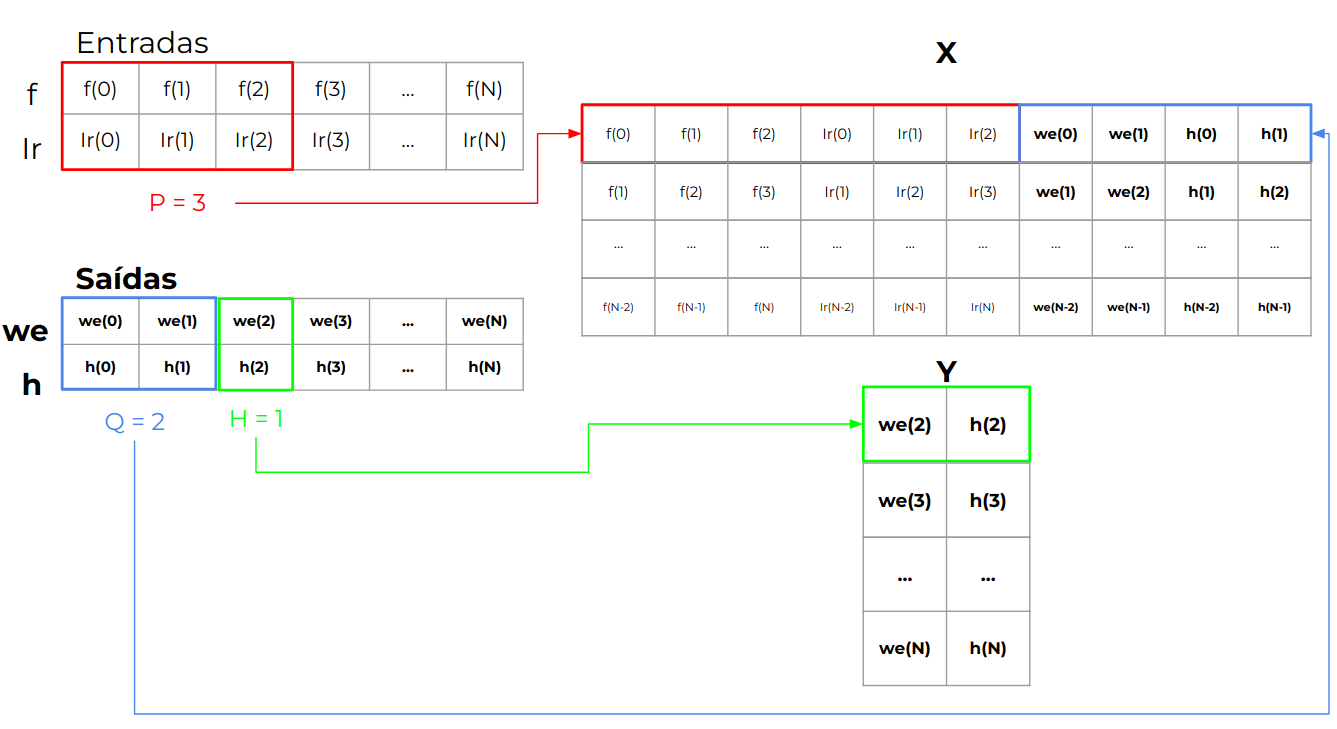
\includegraphics[width=\linewidth]{Imagens/chap03/data_sequencing.png}
    \caption{Sequenciamento dos dados gerados na simulação para $P=3$, $Q=2$ e $H=1$. Fonte: Autor.}
    \label{fig:data_sequencing}
\end{figure}

A influência dos parâmetros $P$, $Q$ e $H$ na performance da identificação da dinâmica serão analisados na seção de Resultados. O \textit{script} contendo as funções que realizam o processamento dos dados está presente em \ref{code:process_data}

\section{Definição da Rede}
\subsection{Arquitetura}
A rede neural neste trabalho foi desenvolvida utilizando o framework \textit{Keras/Tensorflow} em \textit{Python} \cite{tensorflow2015}. Ela consiste em duas camadas:
\begin{enumerate}
    \item Camada LSTM: Nesta camada, foram utilizados 64 células LSTM como a ilustrada na figura \ref{fig:lstm_cell}. A função de ativação utilizada foi a ReLU (Rectified Linear Unit), cuja equação é $f(x) = \max(0,x)$.
    \item Camada MLP: Nesta camada, foram utilizados 2 neurônios clássicos como o ilustrado na figura \ref{fig:mlp_scheme}, com a mesma função de ativação ReLU. A função desta camada é reduzir a dimensão da saída para a mesma das amostras de $Y$, no caso um vetor de 2 elementos ($w_e$ e $h$).
\end{enumerate}
A função de custo utilizada é o MSE, por se tratar de um problema de regressão, e o otimizador utilizado é o Adam \cite{kingma2014adam}, o estado da arte de otimizadores na área de \textit{Deep Learning}, por ser computacionalmente eficiente, ter pouco requisito de memória, ser invariante ao reescalonamento diagonal de gradientes e ser adequado para problemas grandes em termos de dados/parâmetros. A figura \ref{fig:model_summary} ilustra o diagrama de blocos da rede, com as especificações de cada camada.

\begin{figure}[hbt!]
    \centering
    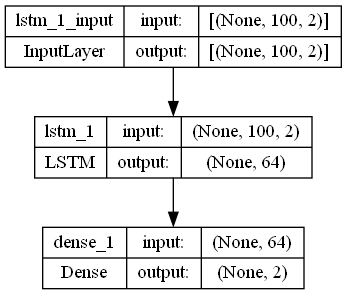
\includegraphics[width=0.4\linewidth]{Imagens/chap03/model_summary.png}
    \caption{Diagrama de blocos da rede neural desenvolvida. Fonte: Autor.}
    \label{fig:model_summary}
\end{figure}

\subsection{Hiperparâmetros do treinamento}
Os hiperparâmetros do treinamento da rede são:
\begin{enumerate}
    \item Número de épocas ($E$): Indica o número de iterações de treinamento da rede.
    \item Tamanho de batelada ($B$): Indica o número de amostras utilizada no treinamento em uma época.
    \item Taxa de validação ($V$): Indica a porcentagem do total de amostras usadas no treinamento que serão utilizadas como validação. 
\end{enumerate}
Para este trabalho, foi utilizado $E=50$, $B=32$ e $V=10\%$. O ajuste desses e dos demais hiperparâmetros foi realizado pelo \textit{script} \ref{code:tune_model}.

\section{Implementação do Controle MPC}
A figura \ref{fig:mpc_loop} ilustra a malha de controle MPC proposta neste trabalho. A rede LSTM é utilizada como o modelo preditivo que será usado pelo otimizador.

\newpage
\begin{figure}[hbt!]
    \centering
    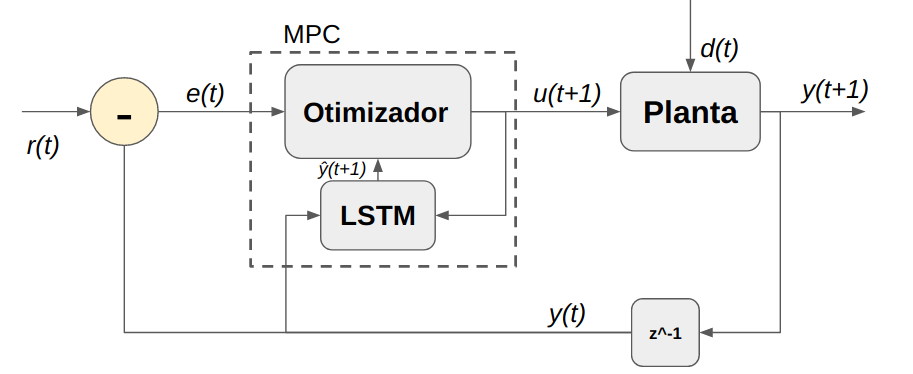
\includegraphics[width=0.8\linewidth]{Imagens/chap03/mpc_loop.png}
    \caption{Malha de controle MPC proposta neste trabalho. Fonte: Autor.}
    \label{fig:mpc_loop}
\end{figure}

\label{sec:mpc_imp}
\subsection{Modelo}
A predição realizada pela LSTM pode ser formulada como:
\begin{equation}
    \hat{y}(t) = g(U_H(t), Y_H(t-1))
\end{equation}
onde $U_H(t)= [u(t), u(t-1), ..., u(t-P+1)] \in \mathcal{R}^{P\times 2}$ é o vetor das entradas passadas e $Y_H(t)=[y(t), y(t-1), ... , y(t-Q+1)] \in \mathcal{R}^{Q \times 2}$ é o vetor de saídas passadas. Este modelo será utilizado dentro do otimizador para modelar as dinâmicas futuras do processo dentro de um horizonte de predição.

\subsection{Otimizador}
A otimização do controle NPMC em questão consiste na minimização de dois erros, o de rastreamento da saída e de regularização da variação de controle, como no exemplo formulado abaixo \cite{yan2022lstm}. A regularização é feita em cima da variação do sinal de controle e não do sinal original, pois é interessante minimizar grandes variações e sobressaltos nos parâmetros de entrada do processo GMAW, para evitar defeitos de fabricação.

\begin{align}
    \min_{U_F(t)} J(t) &= \min_{U_F(t)} a \sum_{k=1}^{N}(r(t+k)-\hat{y}(t+k))^2 + b \sum_{k=1}^{M}\Delta u(t+k)^2 \\
    \text{sujeito a} & \\
    &\hat{y}(t) = g(U_H(t), Y_H(t-1)) \\
    &u_{min} \leq u(t) \leq u_{max} \\
    &\hat{y}_{min} \leq \hat{y}(t) \leq \hat{y}_{max} \\
    & e(t+N) = 0  \\
    & \Delta u(k+M) = 0
\end{align}

onde $M$ e $N$ são os horizontes de controle e predição, respectivamente, $r(t)$ é a trajetória desejada, $a$ e $b$ são os pesos de saída e controle, respectivamente, $U_F(t) = [u(t+1), u(t+2), ... , u(t+M)] \in \mathcal{R}^{M \times 2}$ e $Y_F(t) = [y(t+1), y(t+2), ... , y(t+N)] \in \mathcal{R}^{N \times 2}$, e $\Delta u(t+k) = u(t+k) - u(t+k-1)$. Para instante $t$, calcula-se o controle ótimo $U^*_F(t)$ e utiliza como controle o primeiro ponto. Em suma $u^*(t) = U^*_F(0)$. 

Essa minimização é atingida através de um algoritmo de descida de gradiente (GD) que atualiza $U_F(t)$ de acordo com:

\begin{align}
    U_F^{k+1} &= U_F^k + \Delta U_F^k \\
    \Delta U_F^k &= \eta\left(\frac{\partial J^k}{\partial U_F^k}\right)
\end{align}

onde $\eta > 0$ é a taxa de atualização do otimizador. A Matriz Jacobiana é denotado por
\begin{align} \label{eq:dJdU}
    \frac{\partial J^k}{\partial U_F^k} &= \begin{bmatrix}
        \frac{\partial J}{\partial u(t+1)} \\
        ... \\
        \frac{\partial J}{\partial u(t+M)} 
    \end{bmatrix}
\end{align}

onde o $h$-ésimo elemento da matriz definida em \ref{eq:dJdU} é definido por 
\begin{align}\label{eq:dJdu}
    \frac{\partial J}{\partial u(t+h)} = &-2a\sum_{j=1}^N [r(t+j) - \hat{y}(t+j)] \frac{\partial \hat{y}(t+j)}{\partial u(t+h)} \\
    &+2b\sum_{j=1}^M \Delta u(t+j) \frac{\partial \Delta u(t+j)}{\partial u(t+h)}
\end{align}

O termo $\frac{\partial \Delta u(t+j)}{\partial u(t+h)}$ é expandido em termos da função Delta de Kronecker 
\begin{align}
    \frac{\partial \Delta u(t+j)}{\partial u(t+h)} &= \frac{\partial u(t+j)}{\partial u(t+h)} - \frac{\partial u(t+j-1)}{\partial u(t+h)} \\
    &= \delta(h,j) - \delta(h,j-1)
\end{align}
onde $\delta(h,j)=\begin{cases}
    1 & \text{se } h=j \\
    0 & \text{se } h \neq j
\end{cases}$. 

Já o termo $\frac{\partial \hat{y}(t+j)}{\partial u(t+h)}$ é extraído do modelo LSTM através de uma função própria da biblioteca do $tensorflow$ \cite{tensorflow2015} que calcula via \textit{Backpropagation Trough Time} (BPTT) \cite{lillicrap2019backpropagation}. O detalhamento do algoritmo de estimação de $\frac{\partial \hat{y}(t+j)}{\partial u(t+h)}$ e de $\frac{\partial J^k}{\partial U_F^k}$ estão descritos nos Algoritmos \ref{alg:bptt} e \ref{alg:compute_step}, respectivamente, e presentes no \textit{script} \ref{code:gmaw_mpc}
\newpage
\begin{algorithm}{
    \label{alg:bptt}
    \caption{Extração da matriz Jacobiana}
    \Entrada{$U_H$, $Y_H$, $U_F$}
    \Saida{Matriz Jacobiana $\frac{\partial \hat{y}(t+j)}{\partial u(t+h)}$ i $\in [1, N]$, $j \in [1, i]$}
    k = 1\;\\
    \While{k \leq M}{
        \If{$k < M$}{
            $u(t+k) = U_F(k)$\; \\
        }
        \Else{
            $u(t+k) = u(t+M)$
        }
        Atualiza $U_H(t+k)$ com $u(t+k)$\;
        $x = (U_H(t+k), Y_H(t))$\; \\
        Calcula $\hat{y}(t+k)$ por $g(x(t+k))$\; \\
        Extrai $\frac{\partial \hat{y}(t+k)}{x(t+k)}$\; \\
        $l = 1$\; \\
        \While{h \leq P}{
            $\frac{\partial \hat{y}(t+k)}{u(t+h)} = \frac{\partial \hat{y}(t+k)}{x(t+k)} (P-h) $\; \\
            $h = h+1$ \;
        }
        Atualiza $Y_H(t+k)$ com $\hat{y}(t+k)$\; \\
        $k = k + 1$\;
    }
}
\end{algorithm}

\newpage
\begin{algorithm}{
    \label{alg:compute_step}
    \caption{Otimização do controle $U_F$ via GD}
    \Entrada{$U_F(t)$, $R(t)$, $\frac{\partial \hat{y}(t+j)}{\partial u(t+h)}$ i $\in [1, N]$, $j \in [1, i]$, $a$, $b$ e $\eta$}
    \Saida{$U_F^{k+1}(t)$}
    Calcula $\Delta U_F(t) = [\Delta u_F(t+1), \Delta u_F(t+2), ... , \Delta u_F(t+M)]$\; \\
    Calcula $\frac{\partial \Delta U_F}{\partial U_F}$\;\\
    $j = 1$\; \\
    \While{j \leq M}{
        $\frac{\partial J}{\partial u(t+j)} = -2 \sum_{l=1}^2a_l\left(\sum_{k=1}^{N} [r(t+k)-\hat{y}(t+k)]\frac{\partial \hat{y}(t+k)}{\partial u(t+j)}\right) + 2 \sum_{l=1}^2b_l\left(\sum_{k=1}^{N} \Delta u_F(t+k)\frac{\partial \Delta u_F(t+k)}{\partial u(t+j)}\right)$\; \\
        $u(t+j)^{k+1} = u(t+j)^k -\eta \frac{\partial J}{\partial u(t+j)}$ \; \\
        $j = j + 1$\;
    }
}
\end{algorithm}

Daí, roda-se a simulação utilizando $a=[10,10]$, $b=[1, 1]$, $M=P$, $N=Q$, $\eta=0.1$ e 10 passos de otimização. O algoritmo \ref{alg:mpc_algo} é encarregado da simulação do controle MPC.
\begin{algorithm}{
    \label{alg:mpc_algo}
    \caption{Simulação do controle MPC}
    \Entrada{$R(t)$, $M$, $N$, $a$, $b$, $\eta$, $y(0)$, o tempo total de simulação $T$, a tolerância $\epsilon_{opt}$}
    \Saida{$U^*(t)$}
    Inicializa $Y_H$ e $U_H$\; \\
    Atualiza $Y_H$ com $y(0)$\; \\
    \While{t \leq T}{
        Roda o Algoritmo 1 para extrair $U_F(0)$ e $Y_F(0)$\; \\
        $u^*(1)=u_F(1)$ \; \\
        Atualiza $U_F$ com $u^*(1)$\; \\
        Calcula $y(1)$ através do modelo dinâmico equacionado \; \\
        Atualiza $Y_H$ com $y(1)$\; \\
        $t = t + 1$\; \\
    }
}
\end{algorithm}

\newpage
\subsection{Análise de Estabilidade}
Em geral, garantir a estabilidade de um sistema de controle é de suma importância dentro da teoria de controle. No caso deste trabalho, onde o controle preditivo é realizado através de uma rede neural que modela uma dinâmica não linear (LSTM-NMPC), a estabilidade é investigada checando a monotonicidade da função custo estabelecida, que garante a estabilidade asintótica do controlador.

Assumindo que $U_F(k)$ é ótimo no tempo $k$, estimado pelo otimizador. Agora, introduzindo um controle subótimo $U_Fk+1)$ postulado no tempo $k+1$:
\begin{equation}
    U_F(k+1) = [u(k+1), u(k+2), ... , u(k+M)]^T
\end{equation}

cuja função custo é definida como
\begin{equation}
        \min_{U_F(k+1)} J(k+1) &= \min_{U_F(k+1)} a \sum_{j=1}^{N}(r(k+1+j)-\hat{y}(k+1+j))^2 + b \sum_{j=1}^{M}\Delta u(k+1+j)^2
\end{equation}

\newpage
Com isso, a diferença entre $J(k)$ e $J(k+1)$ é
\begin{align}
    J(k+1) - J(k) &= a[e^2(k+N+1)-e^2(k+1)] - b\Delta u^2(k) = \\
    &= -ae^2(k+1) - b\Delta u^2(k) \leq 0
\end{align}

Portanto, para $a, b > 0$, o custo $J(k)$ é decai monotonicamente com respeito ao tempo e o controle é estável. 